\section{Methods}
%%Muthu: To introduce and motivate context here

\subsection{Software Design}
Based on the user study, we divided the extension into three components: translating, learning and testing. After user opened a news website, 
some words in the main content will be replaced by their translation from user's preferred foreign language, and this is what our translating 
component is doing. If user want to know more about the replaced word, he can simply move his mouse over the translation and a window will pop 
over to help user learn this word, and this is learning component. If user have encountered some word for a few times, we will generate some 
quiz for him and this is testing component.

\begin{figure}[ht]
  \centering
  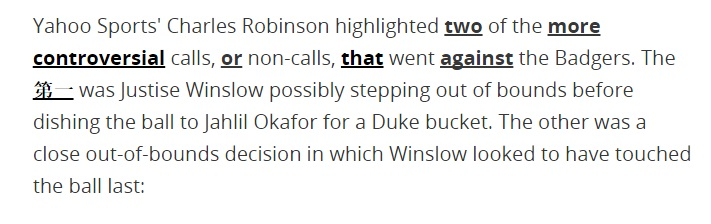
\includegraphics[width=0.45\textwidth]{software_design_2.jpg}
  \caption{Screen shot of Translating Component}
  \label{fig:software_design_2}
\end{figure}
{\bf Translating.} After the original web page, our chrome extension will fetch the content of the news and pass them to the server paragraph by paragraph. After receiving the content, server will compare every word in the paragraph with the words in our vocabulary. If there are some matches, which simply means there are some words that need to be replaced. As every English word might have a few Chinese meanings, our server must select the most appropriate translation among all the meanings. The way that we are trying to solve this problem so far is to compare all the Chinese meanings with the translation of the whole sentence from Bing Translate. If any of the Chinese meanings is the substring of the translation of the sentence, our server will choose that meaning (This is not a proper and accurate way to solve this problem, but it is much better than randomly choose one Chinese meanings. Also, this would be my main research problem that I need to solve next semester). Then, server will pass a JSON string that contains all the words that need to be replaced, their Chinese meanings as well as their pronunciations back to front end. Then, front end will replace the content of the news paragraph by paragraph, in which some words have been replaced. Figure \ref{fig:software_design_2} is the screen shot of this component.

\begin{figure}[ht]
  \centering
    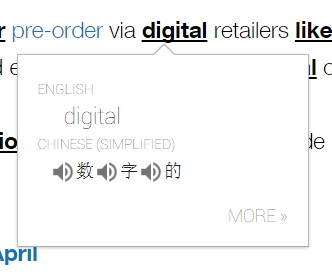
\includegraphics[width=0.3\textwidth]{software_design_4.jpg}
  \caption{Screen shot of popover with highlighted English word}
  \label{fig:software_design_4}
\end{figure}

\begin{figure}[ht]
    \centering
    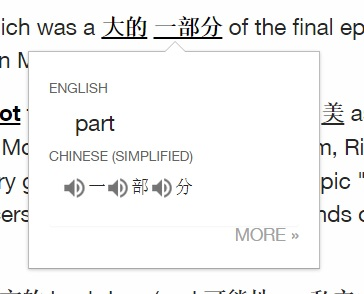
\includegraphics[width=0.3\textwidth]{software_design_5.jpg}
    \caption{Screen shot of popover with highlighted Chinese word}
    \label{fig:software_design_5}
\end{figure}

{\bf Learning.} By moving mouse on the Chinese word for one second, a window with its English meaning and pronunciation will pop over. Figure \ref{fig:software_design_4} is the screen shot of the pop over without its example sentence. If user want to know how to use this word, he can just click the button next to the pronunciation to get the example sentences of this word. After user click the button to get example sentence, our extension will send a request to server and wait for server' response. There is another way of doing this, which is simply get the example sentences together with the words in the Translating component. However, the example sentences contains much more characters comparing with the pronunciation. We want to maximize the loading speed and minimize the data transferred between front end and server, so we decided to split the pop over content into two request. Figure \ref{fig:software_design_5} is the screen shot of the pop over with its example sentences.

\begin{figure}[ht]
\centering
  \centering
  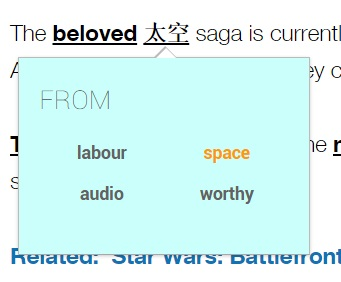
\includegraphics[width=0.3\textwidth]{software_design_7.jpg}
  \caption{Screenshot of English test popover}
  \label{fig:software_design_7}
\end{figure}

\begin{figure}[ht]
    \centering
  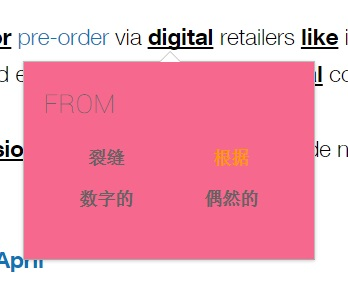
\includegraphics[width=0.3\textwidth]{software_design_8.jpg}
  \caption{Screen shot of Chinese test popover}
  \label{fig:software_design_8}
\end{figure}
{\bf Testing.} When the user has encountered the same word for a few times, our system will generate a quiz about this word for him.  If user move mouse over this replaced word, a window with a quiz will pop over. After user select one option, this window will tell user the correct answer and sent whether the answer is correct to server. Figure \ref{fig:software_design_7} is the screen shot of our testing popover in English. Figure \ref{fig:software_design_8} is the screen shot of our testing popover in Chinese.

{\bf Classifying words category.}
In this section we propose a simple way to classifying words into different categories from online news articles. To find good “category-related” words, it is essential to get the words from those already classified news articles. The following several steps described the approach we used in classifying words category information. The result of this approach is used in generating suitable distractors in Section 5 and as an possible approach in the WSD system discussed in Section 4. 

{\bf Crawling news content.}
Several web crawlers are designed to get news contents from news websites. The crawler will detect URLs from each news website’s main page as and its sub-category pages. For example, there are sub-categories like “football”, “basketball” under main category “Sports”, and the crawler is able to crawl URLs from “football” page and “basketball” page as well. 

After detailed comparison of most news websites, we divided news articles into seven categories, namely “World”, “Technology”, “Sports”, “Entertainment”, “Finance”, “Health” and “Travel”. Most news articles can be classified into one of the seven categories. The web crawler will store all paragraph tags from each websites and store them as one file under one category. 

{\bf Preprocessing.}
In this step the server uses Natural Language Tool Kit \cite{edw09} for word tokenizing and POS Tagging. The server will store the POS tag of each word. After elimination of all non-English words and those words that contain special symbols, like ``O’Real", ``S\$40", all words that contains only alphabetic letters are conserved. All stop words are also eliminated as well. They are stored as lower case for the ease of future process.

{\bf Classification.}
In the classification step, the server counts the document frequency of each word in all those stored news articles, i.e. if word “scored” appeared 4 times in one article, it will only be counted as once. By following this approach we can successfully reduce the bias of some words only appear a lot of times in one article while don’t appear often in other article. As we are storing similar number of articles in each category, this approach will provide a fair comparison of each word’s popularity among different categories. After this step we will know the document frequency count of each word in different category. 
Assume C is the list of category names, and f(w, C(i))=m means word w appeared in category C(i) for m times, then the sum weight of word w as sw(w) is calculated in Equation~\ref{equation:Distractor_1}:

\begin{equation}
sw (w) = \sum_{i=1}^{n} f(w,C(i))
\label{equation:Distractor_1}
\end{equation}  

A word w is classified into category C(i) if it satisfies Equation~\ref{equation:Distractor_3}::

\begin{equation}
f (w, C(i)) - sw(w)/n >= \delta
\label{equation:Distractor_3} 
\end{equation}  

The confidence factor $\delta$ can be a positive integer between 0 and the average number of articles in each category. It means on average, the word w must appear in a specific category C(i) $\delta$ times more than it appear in other category before it can be classified into category C(i).

It is obvious that a higher confidence factor value will result in less number words getting classified, but it will result in getting words that are more accurate. A suitable confident value is selected to generating category-related words in the later section.





